

\chapter{Konstruktion und Design}
\label{chap:konstruktion}


\section{Strukturelles Design des autonomen Segelschiffs}
\subsection{Plaungsprozess mittels CAD}
Computer Aided Design (CAD) ist eine form des technischen Zeichens, welches einem ermöglicht Modelle in Drei dimensionalen Raum zu gestalten. Im Vergleich zum "normalen" 3D modelling arbeitet man mit CAD mit festen Grössen und Masseinheiten. Somit lassen ist es verhältnissmässig einfach Technische Zeichnungen anzufertigen. Es gilt als eines der Wichtigsten Werkzeuge zur Planung von Maschienen und Produkten da sich gewisse Struktur- und Materialialeigenschaften, je nach Applikation, simulieren lassen. Die Konstruktion dieses Projekt begann mit dem erlernen von den Programmen Autodesk Inventor und Autodesk Fusion360. 
Beide Programme verfolgen einen ähnlichen Ansatz und sind ähnlich Aufgebaut. Im Vergleich zu Inventor ist Fusion deutlich nutzerfreundlicher und ermöglicht es Projekte über die Cloud einfacher gebaut. Die Wahl Autodesk zu verwenden ist hauptsächlich dem verschudet, dass Autodesk kostenlose Lizenzen für nicht komerzielle oder Bilungszwecke vergibt.
Alternativen welche jedoch aufgrund des letzten Punktes nicht verwendet wurden sind NX Siemens und Solidworks. 
Eine andere Alternative wäre FreeCAD gewesen, welches sogar mit OpenSource ist. Dem Programm selber fehlen leider einige Funktionen was zur finalen Wahl geführt hat


\subsection{Iterationen}
Wie bereits erwähnt wurde das Schiff so konstruiert, dass es mögliche, starke Krafteinwirkungen standhalten könnte. Daher wurde auf die Interne Kraftverteilung stark geachtet.
\subsubsection{Rippenmuster und dessen Besfestigung}
Ein Rippenmuster, wie es bei Holzbooten üblich ist, wurde verwendet um die Form zu bestimmen. Diese wurden mit einem Geringen Abstand von (Länge einfügen) Plaziert um auch bei seitlichen Krafteinwirkungen genügend Strukturelle stütze zu sein.

\begin{figure}[htb]
  \centering
  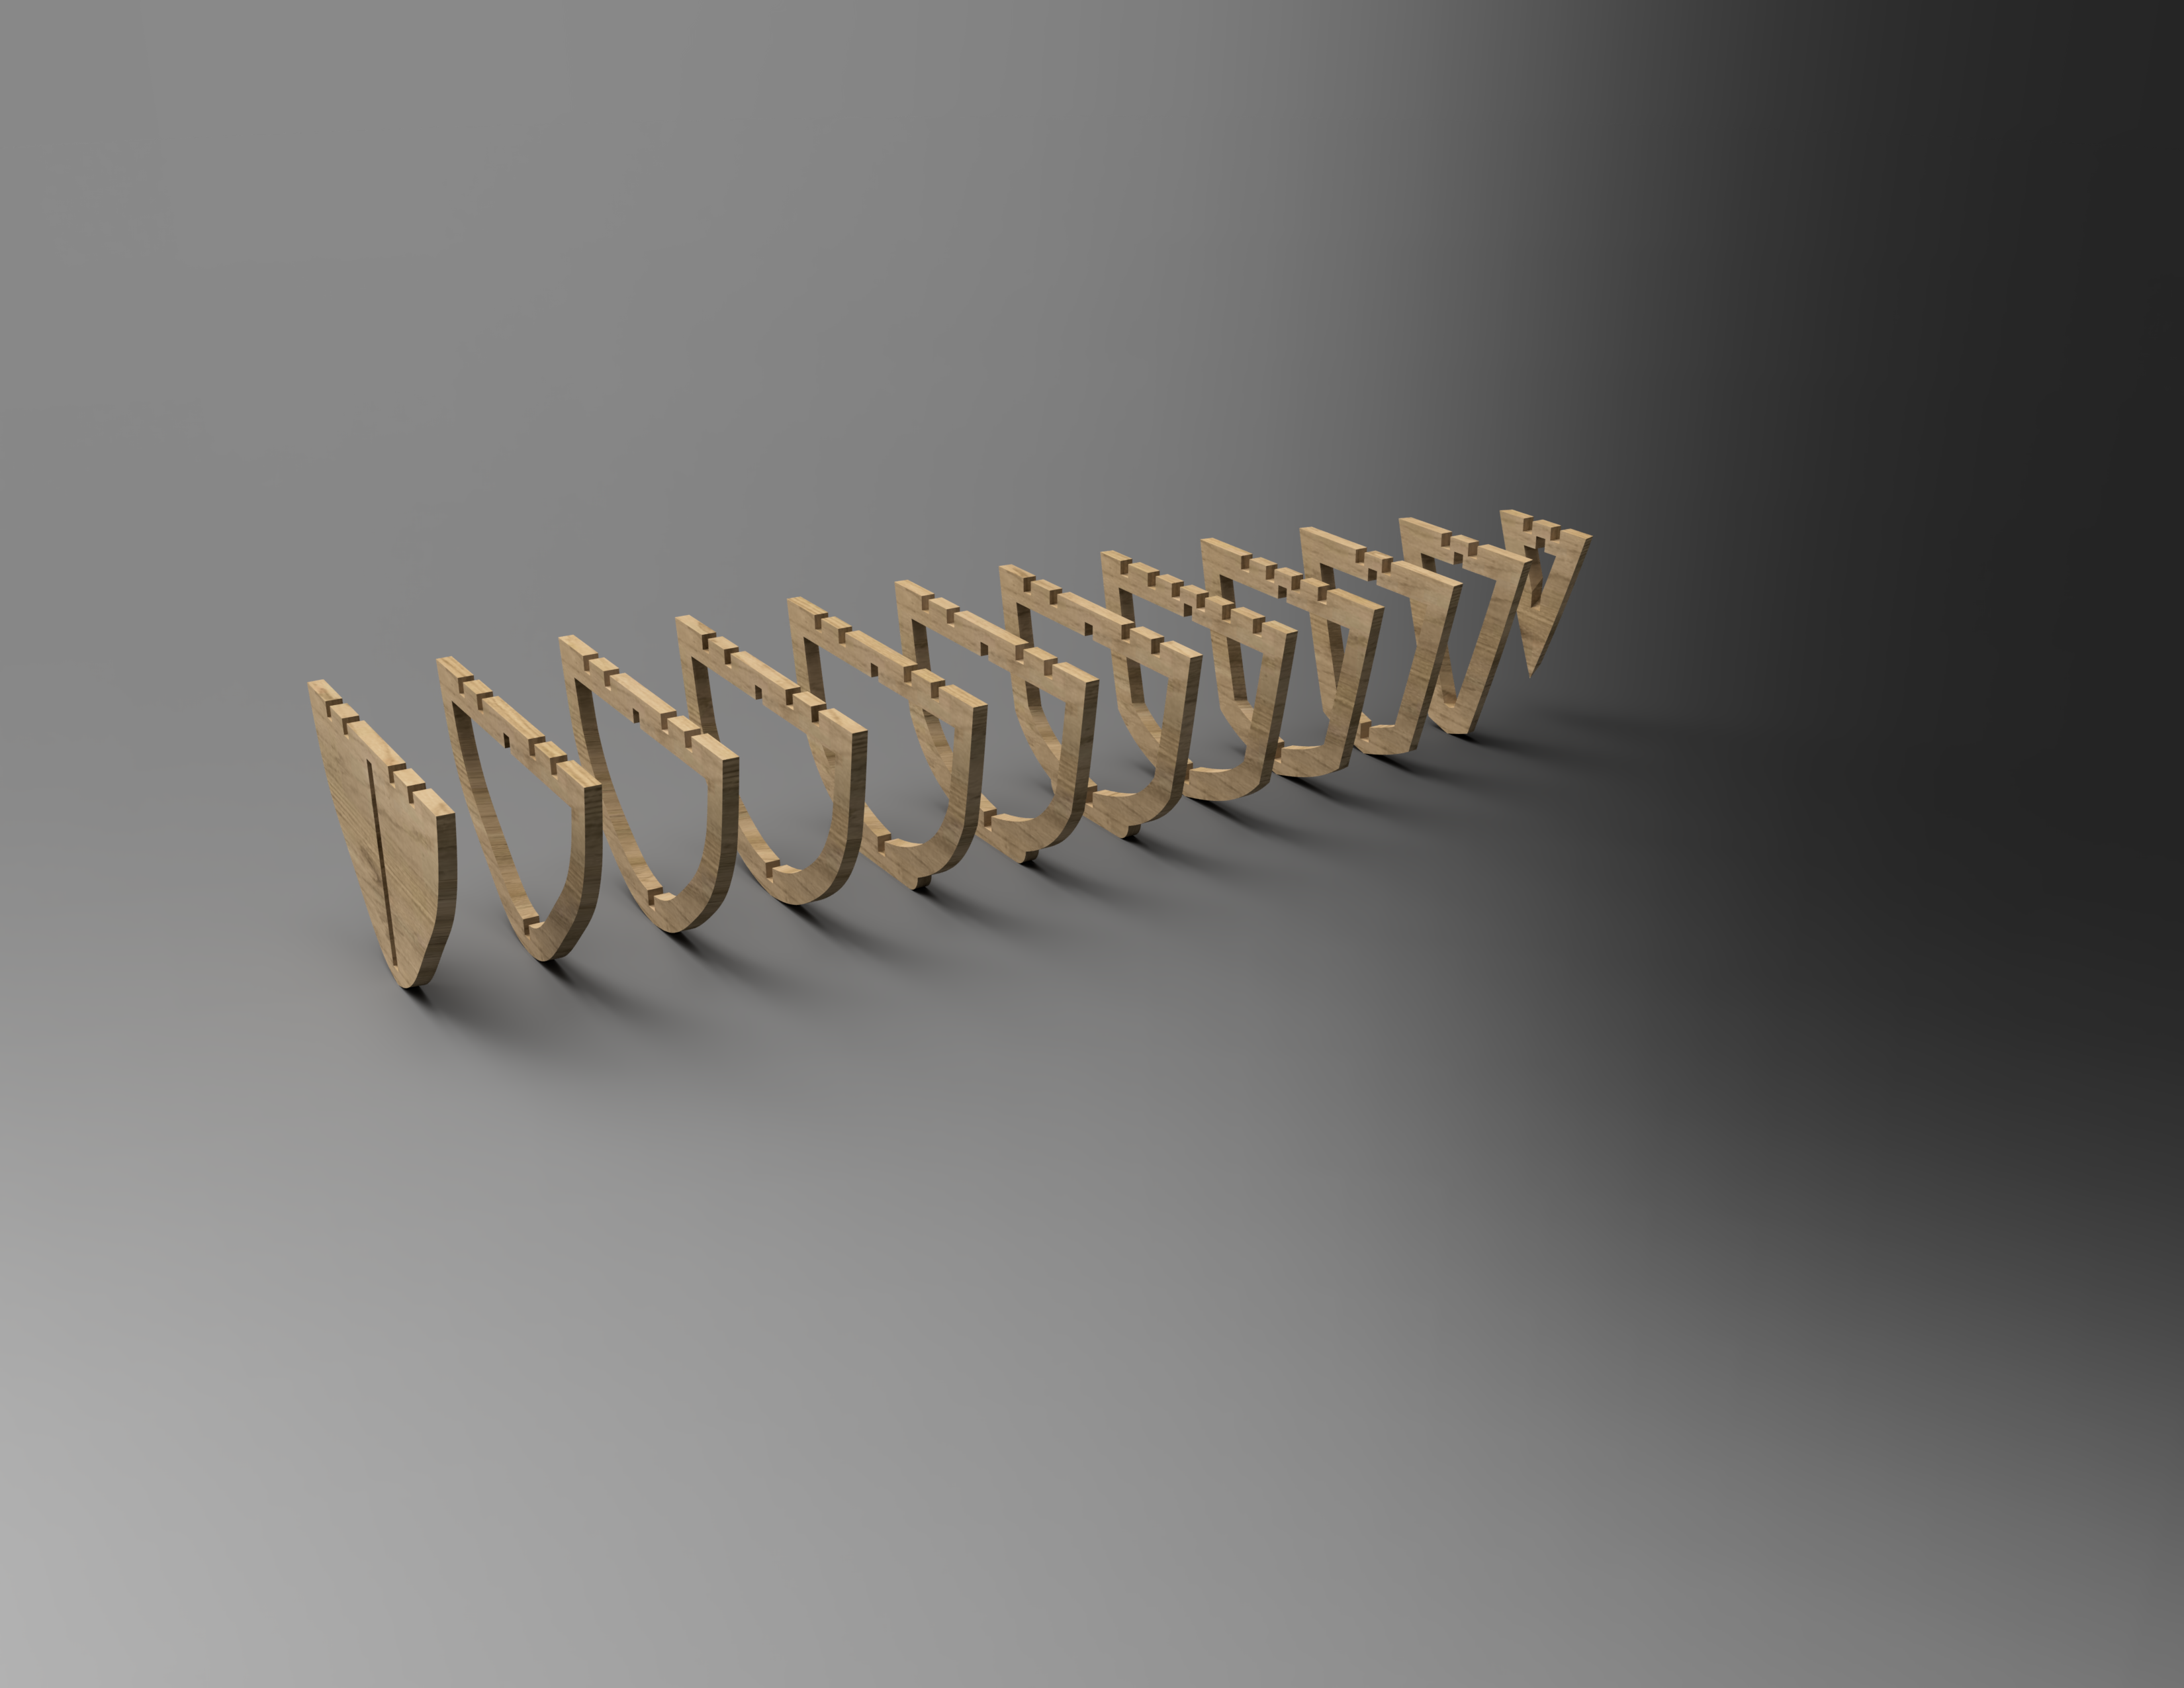
\includegraphics[width=\textwidth]{assets/rippenv1.png}
  \caption{Render einer ersten Version des Rippenmusters }
  \label{fig:rippenv1}
\end{figure}


\section{Materialauswahl und -begründung }

\section{Segel und Sailflap-Implementierung }
\section{Energieversorgung}